\subsubsection{Interfaz de usuario}

En la pantalla principal de la interfaz se muestra un mapa interactivo del entorno, con una cuadrícula que representa el mapa. La interfaz muestra información en tiempo real sobre la celda actual en la que se ubica el robot en el mapa, actualizándose conforme el robot se desplaza. Además, se proporciona información sobre la dirección de movimiento.

El usuario comienza estableciendo los puntos de inicio y destino haciendo click en las celdas disponibles. Cuando se da la orden de inicio, se calcula la ruta óptima y se envían los comandos al robot. Paso seguido, la interfaz muestra continuamente en tiempo real la celda del robot y se envían los comandos de movimiento hacia las celdas subsiguientes.

\begin{figure}[H]
    \centering
    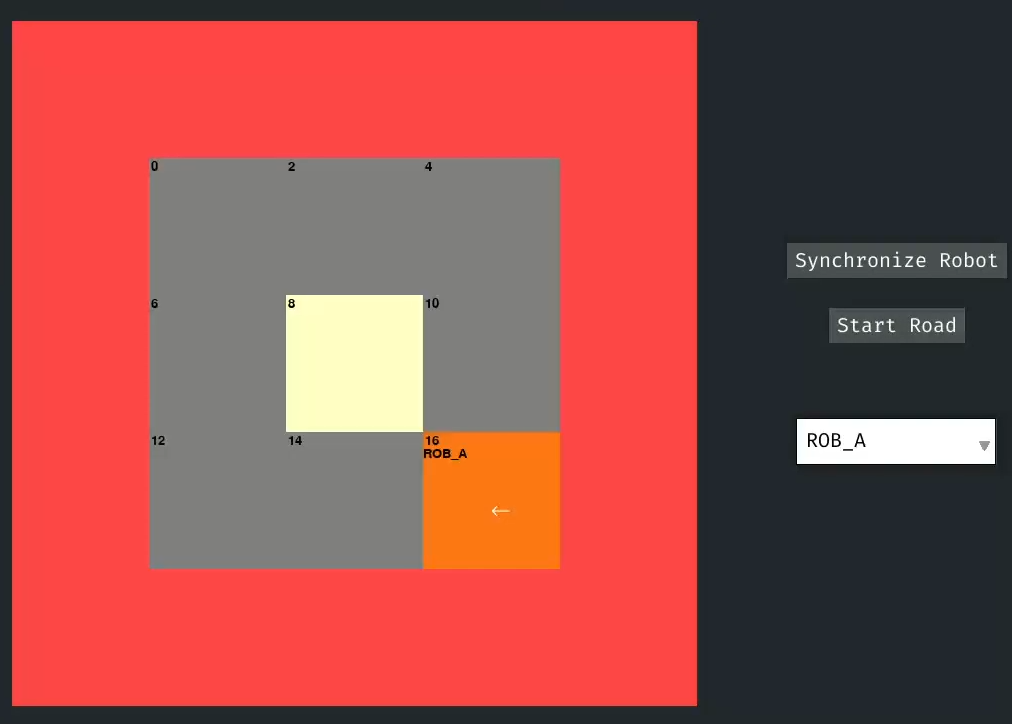
\includegraphics[width=0.85\linewidth]{images/interfaz_de_usuario}
    \caption{Interfaz de usuario}
    \label{fig:interfazusuario}
\end{figure}

